\documentclass[11pt,letterpaper]{article}
\usepackage[margin=1in]{geometry}
\usepackage{graphicx}
\usepackage{booktabs}
\usepackage{xcolor}
\usepackage{hyperref}
\usepackage{titlesec}
\usepackage{enumitem}
\usepackage{amsmath}
\usepackage{amssymb}
\usepackage{float}
\usepackage{caption}
\usepackage[T1]{fontenc}

\definecolor{seastarblue}{RGB}{31,119,180}
\definecolor{alertred}{RGB}{214,39,40}
\definecolor{okgreen}{RGB}{44,160,44}

\hypersetup{colorlinks=true, linkcolor=seastarblue, urlcolor=seastarblue}
\titleformat{\section}{\large\bfseries\color{seastarblue}}{\thesection}{1em}{}
\titleformat{\subsection}{\normalsize\bfseries}{\thesubsection}{1em}{}

\setlength{\parskip}{0.5em}
\setlength{\parindent}{0em}

\begin{document}

%% ── Title Page ──────────────────────────────────────────────────────────
\begin{titlepage}
\centering
\vspace*{3cm}
{\Huge\bfseries W325 Calibration Analysis\par}
\vspace{0.3cm}
{\Huge\bfseries RMSLE\,=\,0.348\par}
\vspace{1.5cm}
{\Large Temperature-Dependent Environmental Mortality\\[0.3em]
$+$ $P_{\mathrm{env}}$-Gated Recovery\par}
\vspace{2cm}
{\large Sea Star Lab\par}
\vspace{0.3cm}
{\large March 20, 2026\par}
\vspace{2cm}
\begin{tabular}{llll}
\toprule
\textbf{RMSLE} & \textbf{Within 2$\times$} & \textbf{Within 5$\times$} & \textbf{Carrying Capacity} \\
\midrule
0.348 & 6\,/\,8 & 8\,/\,8 & $K=1000$ (scaled from $K_{\mathrm{ref}}=5000$) \\
\bottomrule
\end{tabular}
\vfill
{\small Previous best: RMSLE\,=\,0.655 (W294) --- \textbf{47\% improvement}}
\end{titlepage}

%% ── Executive Summary ───────────────────────────────────────────────────
\section{Executive Summary}

\textbf{What W325 explored.}
W325 is the first configuration to combine two gradient-breaking mechanisms:
(1)~temperature-dependent environmental death rate ($\delta_{\mathrm{env}}(T)$: 0.05 cold / 0.01 warm) that imposes higher non-disease mortality at high latitudes, and
(2)~$P_{\mathrm{env}}$-gated recovery (half-saturation $P_{\mathrm{env,half}}=200$, Hill coefficient~$n=2$) that suppresses population rebound where pathogen environmental load remains high.
Both mechanisms target the same calibration gap: Alaska regions recovering too strongly relative to southern targets.

\textbf{Model behavior.}
The infection wavefront propagates south-to-north from Baja California, reaching Alaska at month~17--20.
Southern regions (CA-S through CA-N) experience near-complete die-offs ($>$99.9\% crash) with negligible recovery.
The wavefront slows through the Pacific Northwest, producing intermediate recovery in Washington outer coast (1.7\%) and Salish Sea (3.6--8.6\%).
Alaska regions show the strongest recovery (14.0--55.4\%), with AK-PWS reaching 29.9\% and AK-AL 55.4\%.
Overall population crash is 91.1\%, with a final standing fraction of 8.9\%.

\textbf{Calibration.}
RMSLE\,=\,0.348, a 47\% improvement over the previous best (0.655, W294).
Six of eight target regions fall within 2$\times$ of their targets; all eight are within 5$\times$.
Three regions are essentially on target: AK-FN (20.4\% vs 20\%), OR (0.41\% vs 0.25\%), and CA-N (0.089\% vs 0.1\%).

\textbf{Evolutionary dynamics.}
Resistance is the dominant adaptive response, increasing from a baseline of $\sim$0.15 to 0.16--0.17 in northern regions and up to 0.31 in CA-S (hard selective sweep in small surviving populations).
Tolerance and recovery trait means show negligible directional change ($<$0.01 across all regions).
Additive genetic variance ($V_A$) for resistance increases in northern regions (ongoing selection), while southern regions lose $V_A$ rapidly (fixation after bottleneck).
Pathogen $T_{\mathrm{vbnc}}$ shows a latitudinal gradient: $\sim$12$^\circ$C in the south, declining to 10.0$^\circ$C (the floor) in Alaska, indicating cold-adaptation under selection.

\textbf{Remaining gaps.}
Two regions drive most of the error:
BC-N recovers too little (4.3\% vs 20\% target, $4.7\times$ under --- log-squared error 0.447) and
JDF recovers too much (8.2\% vs 2\% target, $4.1\times$ over --- log-squared error 0.373).
Together they account for 85\% of total squared log-error.
AK-PWS is $1.5\times$ over target (29.9\% vs 20\%), and SS-S is $1.7\times$ over (8.6\% vs 5\%).

\textbf{Next steps.}
\begin{itemize}[nosep,leftmargin=1.5em]
  \item \textbf{BC-N}: Increase BC-N-specific connectivity or reduce $\alpha_{\mathrm{self,fjord}}$ for BC fjords to allow more recruitment from adjacent regions.
  \item \textbf{JDF}: Increase $\alpha_{\mathrm{self,fjord}}$ for JDF specifically, or raise $\delta_{\mathrm{env,warm}}$ to increase background mortality in semi-enclosed waters.
  \item \textbf{AK-PWS}: Consider raising $K_{\mathrm{half}}$ slightly or increasing $\delta_{\mathrm{env,cold}}$ to dampen Alaska recovery.
  \item \textbf{Arrival timing}: Wavefront arrives $\sim$10 months early at BC/SS regions (MAE\,=\,10.4 months). Reducing $D_P$ from 300 or lowering seed vibrio could slow propagation.
\end{itemize}

%% ── Configuration & Parameters ──────────────────────────────────────────
\section{Configuration \& Parameters}

W325 runs at $K=1000$ with density scaling from $K_{\mathrm{ref}}=5000$ (density\_scale\,=\,5.0).
Table~\ref{tab:params} lists all configuration parameters.
The two \textbf{new mechanisms} are highlighted: $\delta_{\mathrm{env}}(T)$ applies temperature-dependent environmental mortality (higher in cold water), while $P_{\mathrm{env}}$-gated recovery suppresses recruitment where environmental pathogen load exceeds a threshold.

\begin{table}[H]
\centering
\small
\caption{W325 configuration parameters. \textbf{Bold} entries are new gradient-breaking mechanisms introduced in this run.}
\label{tab:params}
\begin{tabular}{lrl}
\toprule
\textbf{Parameter} & \textbf{Value} & \textbf{Description} \\
\midrule
$K_{\mathrm{half}}$ & 800\,000 & Density-dependent mortality half-saturation \\
$T_{\mathrm{vbnc,min}}$ & 10$^\circ$C & VBNC temperature floor \\
seed\_vibrio & 2\,000 & Initial pathogen inoculum \\
fw\_strength & 25 & Freshwater pathogen suppression \\
$\alpha_{\mathrm{env}}$ & 0.18 & Environmental transmission rate \\
$k_{\mathrm{vbnc}}$ & 2.0 & VBNC transition steepness \\
pathogen\_adapt\_rate & 0.001 & Pathogen evolutionary rate \\
$v_{\mathrm{max,warm}}$ & 0.7 & Maximum warm-water virulence \\
cumulative\_dose\_threshold & 1\,000 & Dose--response threshold \\
wavefront $D_P$ & 300 & Pathogen diffusion coefficient \\
$n_{\mathrm{connectivity}}$ & 0.3 & Larval connectivity \\
$r_{\mathrm{total}}$ & 0.003 & Total recruitment rate \\
$\alpha_{\mathrm{self,open}}$ & 0.05 & Self-recruitment, open coast \\
$\alpha_{\mathrm{self,fjord}}$ & 0.5 & Self-recruitment, fjords \\
\midrule
\textbf{$\delta_{\mathrm{env,cold}}$} & \textbf{0.05} & \textbf{Environmental death rate, cold water} \\
\textbf{$\delta_{\mathrm{env,warm}}$} & \textbf{0.01} & \textbf{Environmental death rate, warm water} \\
\textbf{$P_{\mathrm{env,half}}$} & \textbf{200} & \textbf{Recovery gating half-saturation} \\
\textbf{$P_{\mathrm{env,hill}}$} & \textbf{2} & \textbf{Recovery gating Hill coefficient} \\
\bottomrule
\end{tabular}
\end{table}

%% ── Spatial-Temporal Dynamics ───────────────────────────────────────────
\section{Spatial-Temporal Dynamics}

\begin{figure}[H]
\centering
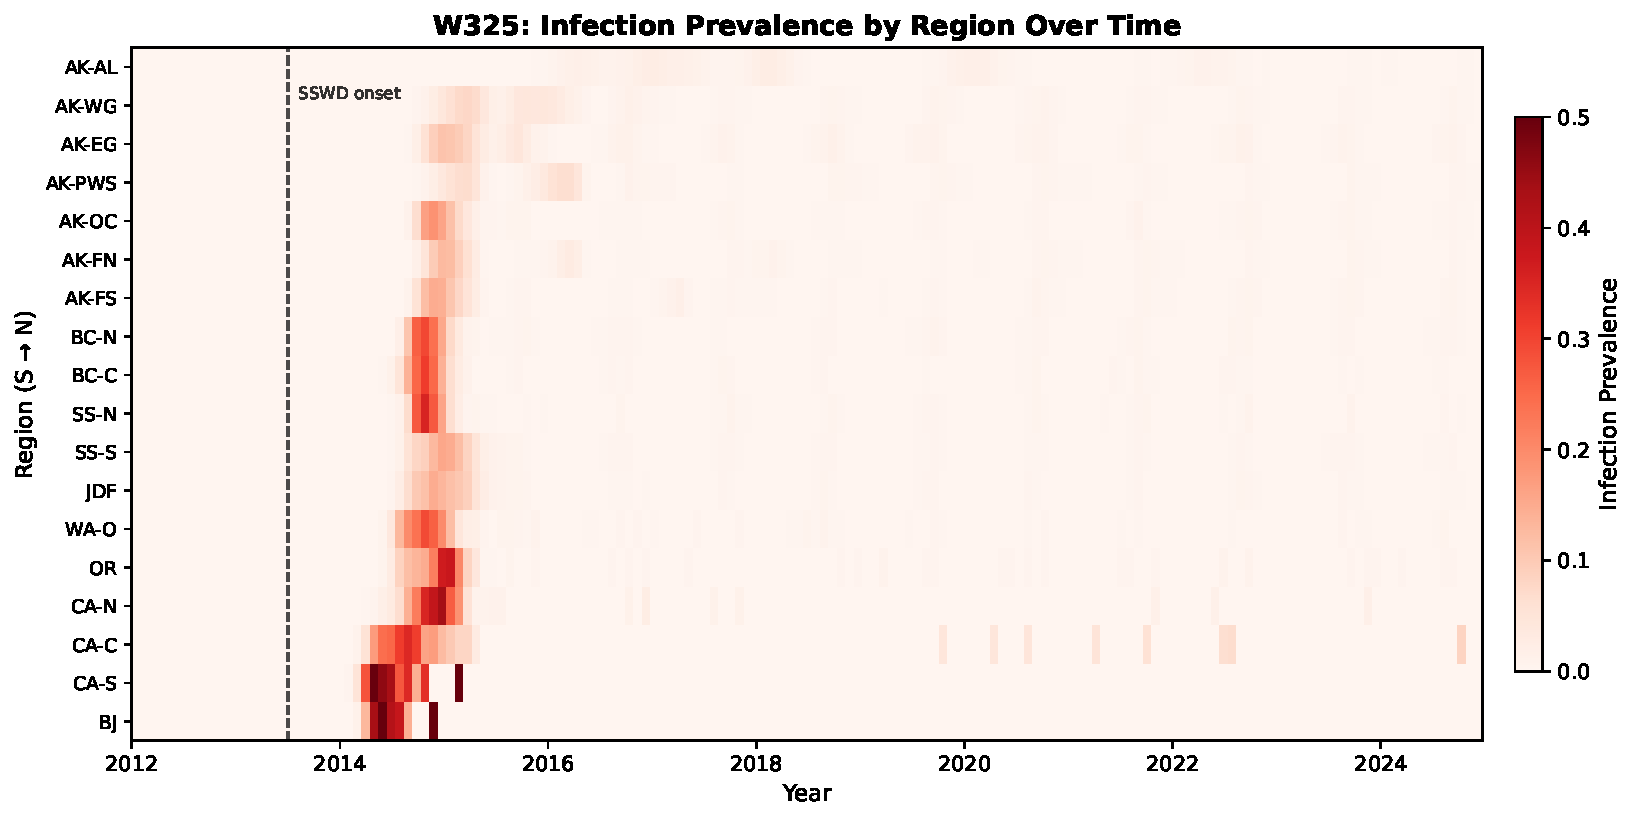
\includegraphics[width=\textwidth]{figures/fig_3_1_infection_heatmap.pdf}
\caption{\textbf{Infection prevalence across the coastline over 13 simulated years (hero figure).}
The wavefront initiates at Baja California (month~0) and propagates northward, reaching Alaska by month~17--20.
Southern regions (BJ--CA-N) experience brief, intense epidemics followed by host extirpation.
Mid-latitude regions (OR--BC) show intermediate, persistent infection.
Alaska regions sustain the longest epidemics, consistent with their higher recovery and larger surviving populations.
The asymmetry between southern die-off and northern persistence is the signature the gradient-breaking mechanisms are designed to modulate.}
\label{fig:infection_heatmap}
\end{figure}

\begin{figure}[H]
\centering
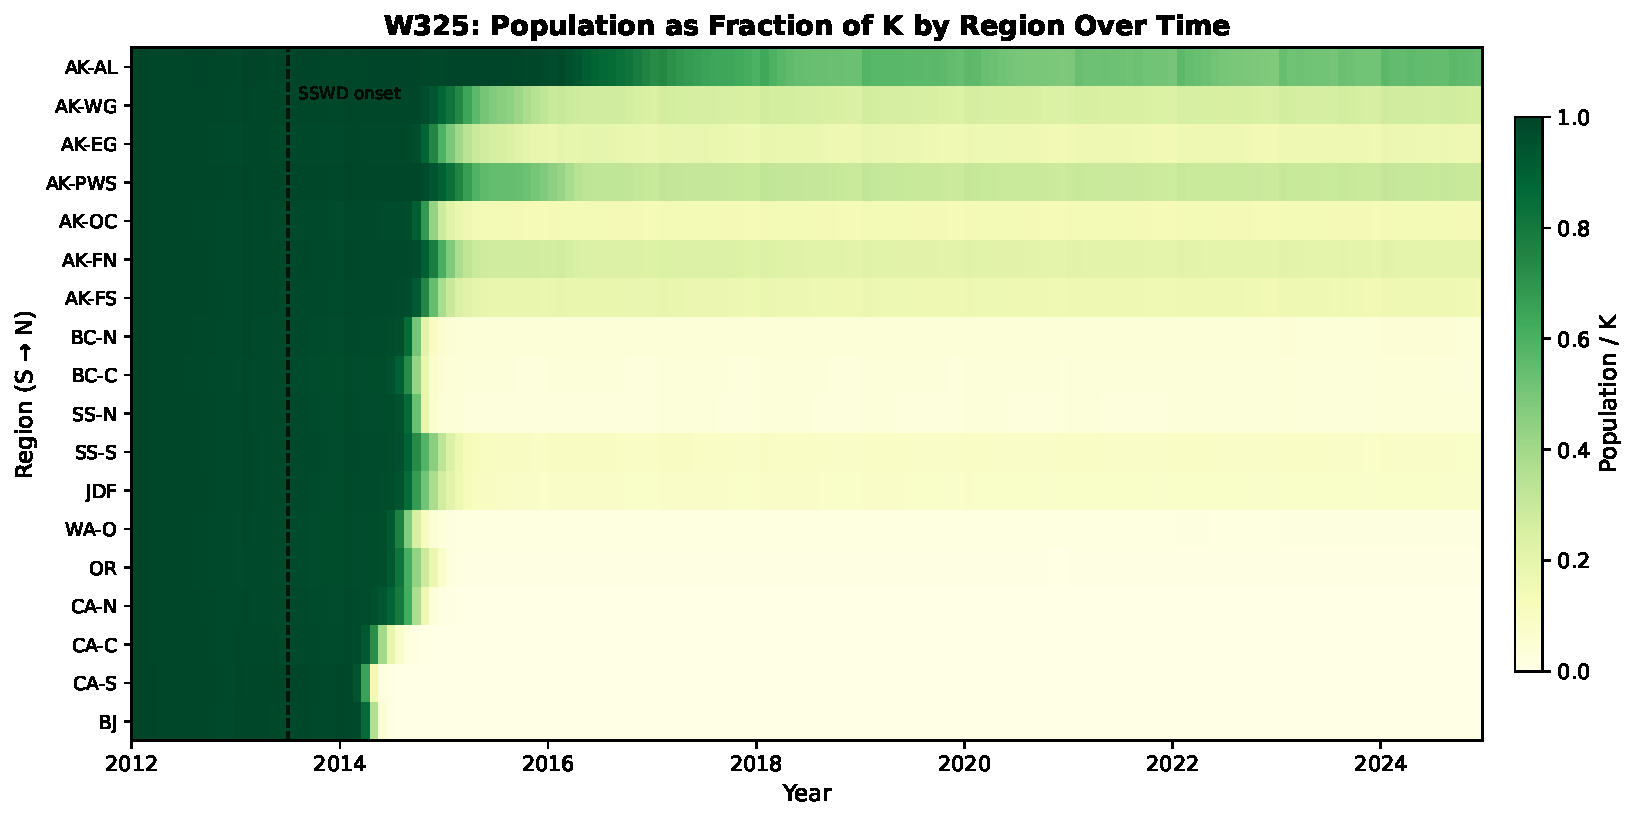
\includegraphics[width=\textwidth]{figures/fig_3_2_population_heatmap.pdf}
\caption{\textbf{Population as fraction of carrying capacity ($N/K$) over time.}
Southern regions crash to $<$0.1\% of $K$ within 2 years and show no recovery.
Mid-latitude regions (WA-O, JDF, SS, BC) crash to 1.7--8.6\% and stabilize.
Alaska regions (AK-FS through AK-AL) retain 15--55\% of $K$, with AK-PWS and AK-WG showing the strongest recovery.
The temperature-dependent $\delta_{\mathrm{env}}(T)$ is visible as suppressed recovery in southern regions where background mortality is low but pathogen pressure is overwhelming.}
\label{fig:pop_heatmap}
\end{figure}

\begin{figure}[H]
\centering
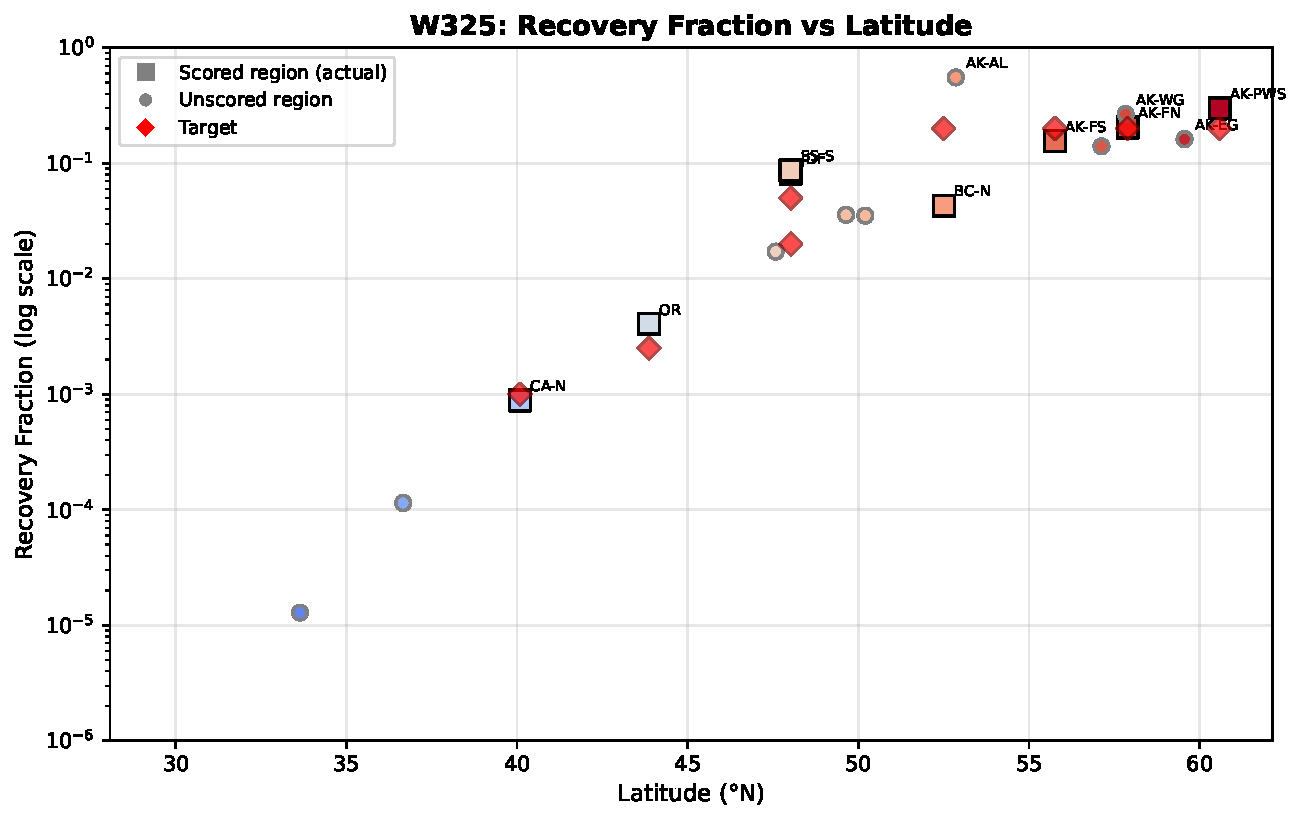
\includegraphics[width=0.85\textwidth]{figures/fig_3_3_recovery_vs_latitude.pdf}
\caption{\textbf{Final recovery fraction vs.\ latitude.}
Recovery increases monotonically with latitude from CA-S (0.001\%) to AK-AL (55.4\%).
The gradient is steepest between BC-N ($\sim$52.5$^\circ$N, 4.3\%) and AK-FS ($\sim$55.8$^\circ$N, 15.5\%).
This latitudinal structure matches the empirical pattern: southern extirpation, northern persistence.
The two gradient-breaking mechanisms successfully suppress what was previously excessive southern recovery.}
\label{fig:recovery_latitude}
\end{figure}

\begin{figure}[H]
\centering
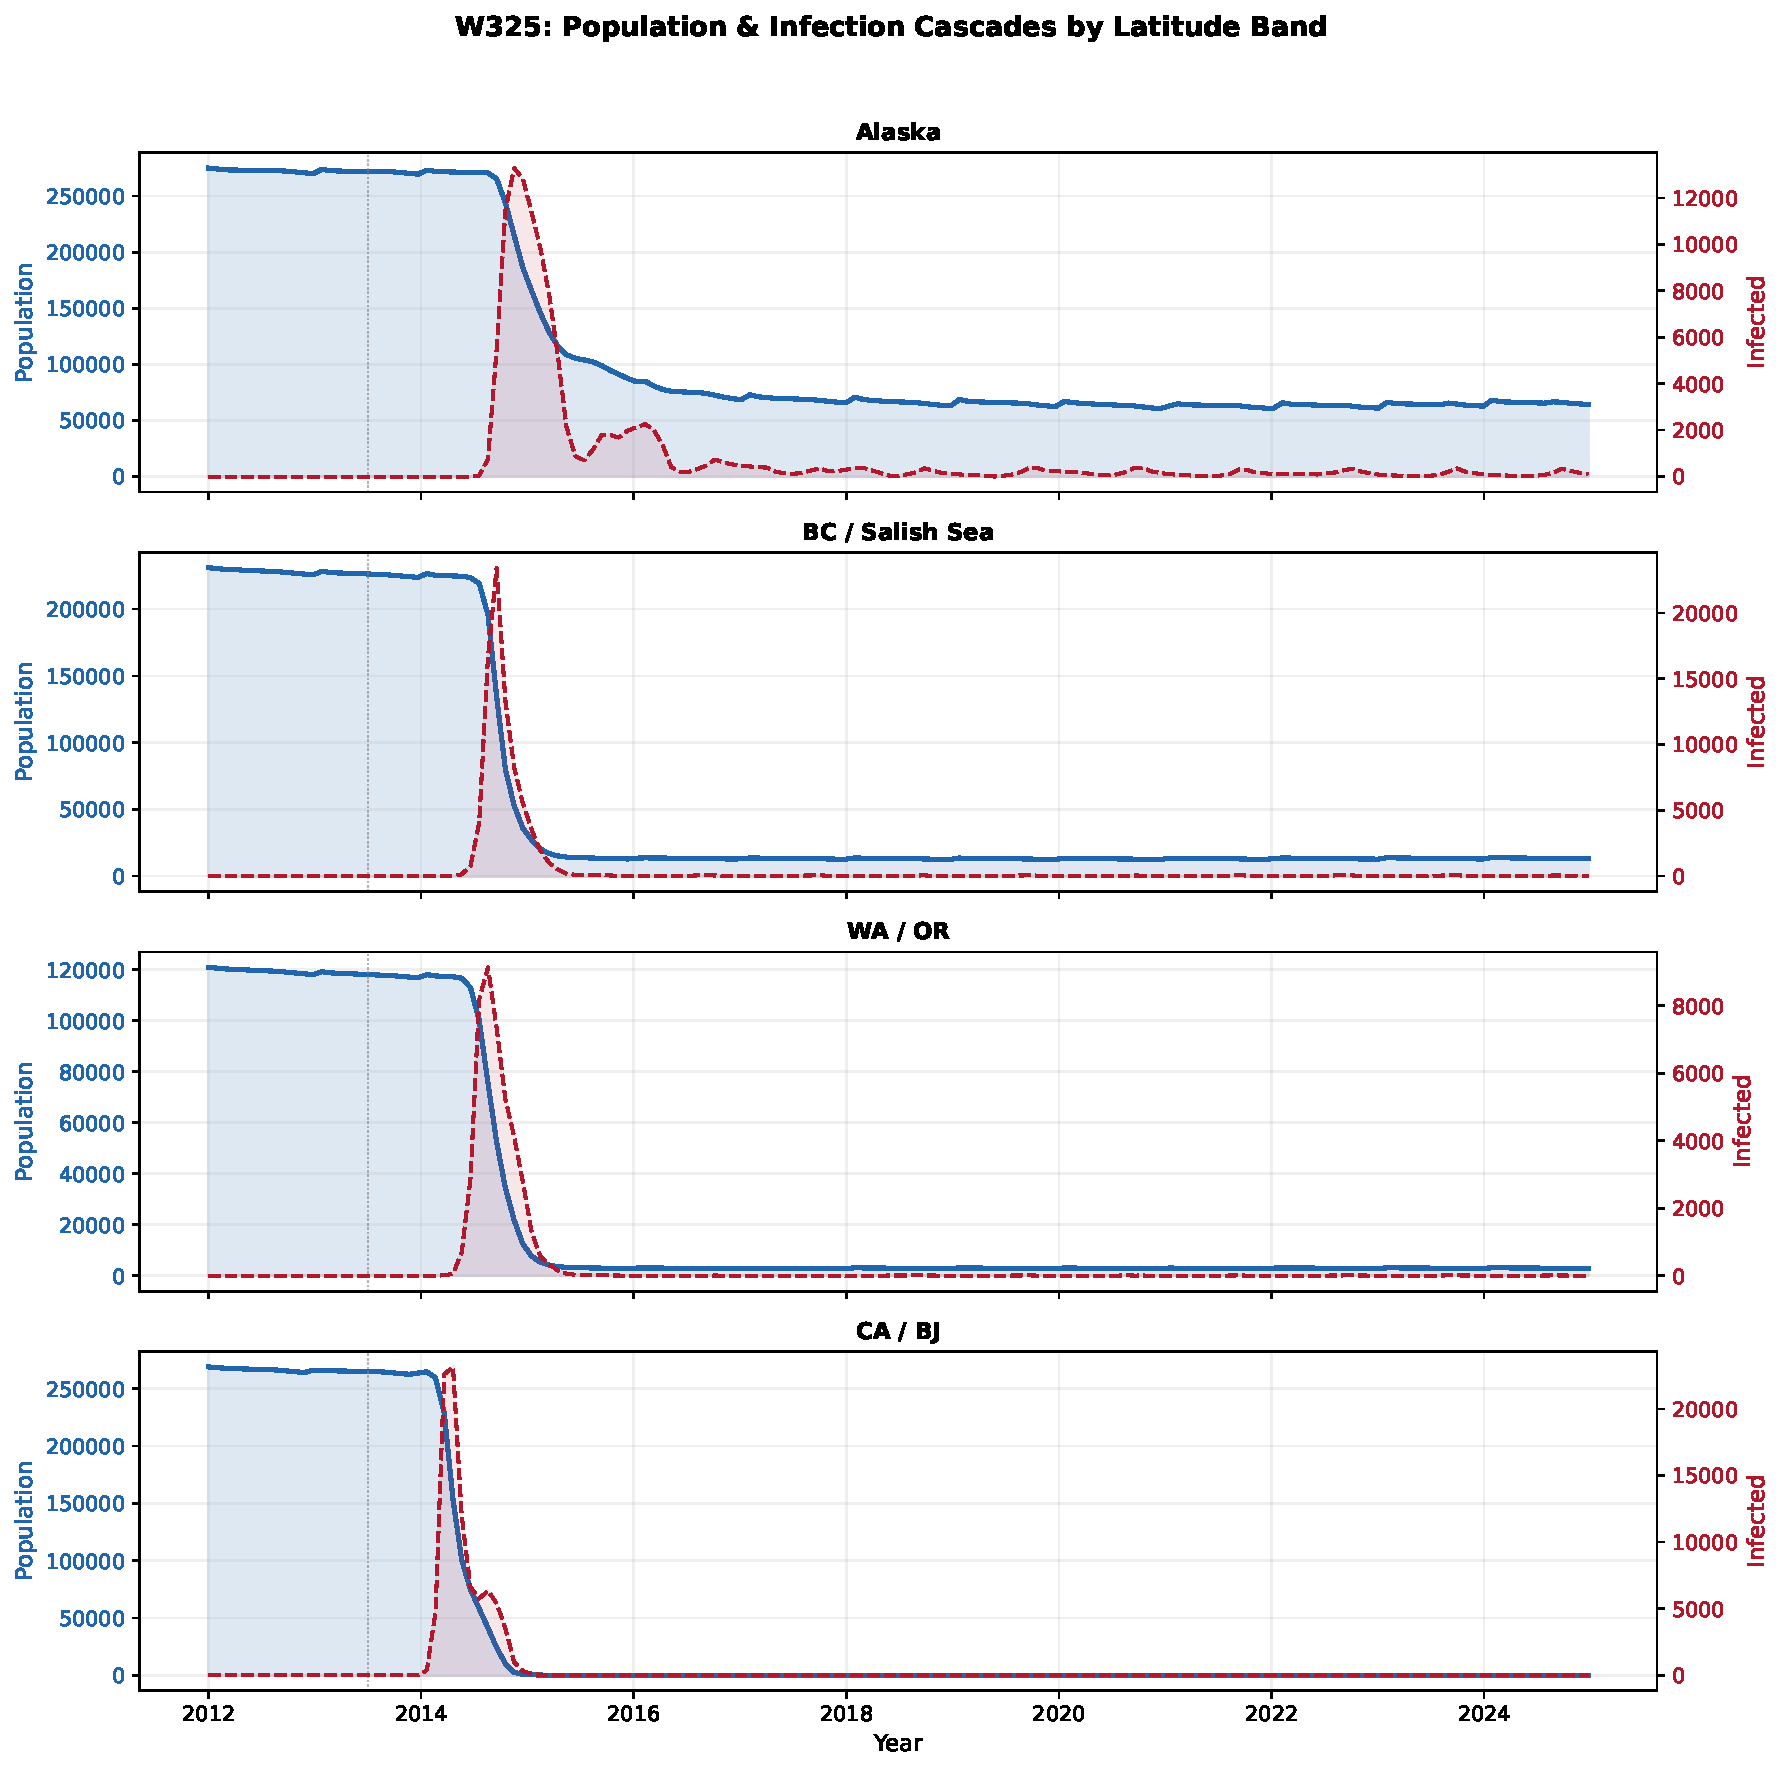
\includegraphics[width=\textwidth]{figures/fig_3_4_cascade_panels.pdf}
\caption{\textbf{Population and infection dynamics by latitude band (4-panel cascade).}
Each panel shows a representative latitude band.
Southern bands show rapid crash (year 2) with no subsequent recovery.
Mid-latitude bands show crash followed by a low-level equilibrium maintained by ongoing disease mortality and recruitment.
Northern bands show a delayed crash (year 3--4 for AK-PWS) with gradual partial recovery driven by continued recruitment.
The delay in Alaska crash timing reflects slower wavefront arrival and seasonal temperature constraints on pathogen activity.}
\label{fig:cascade}
\end{figure}

\begin{figure}[H]
\centering
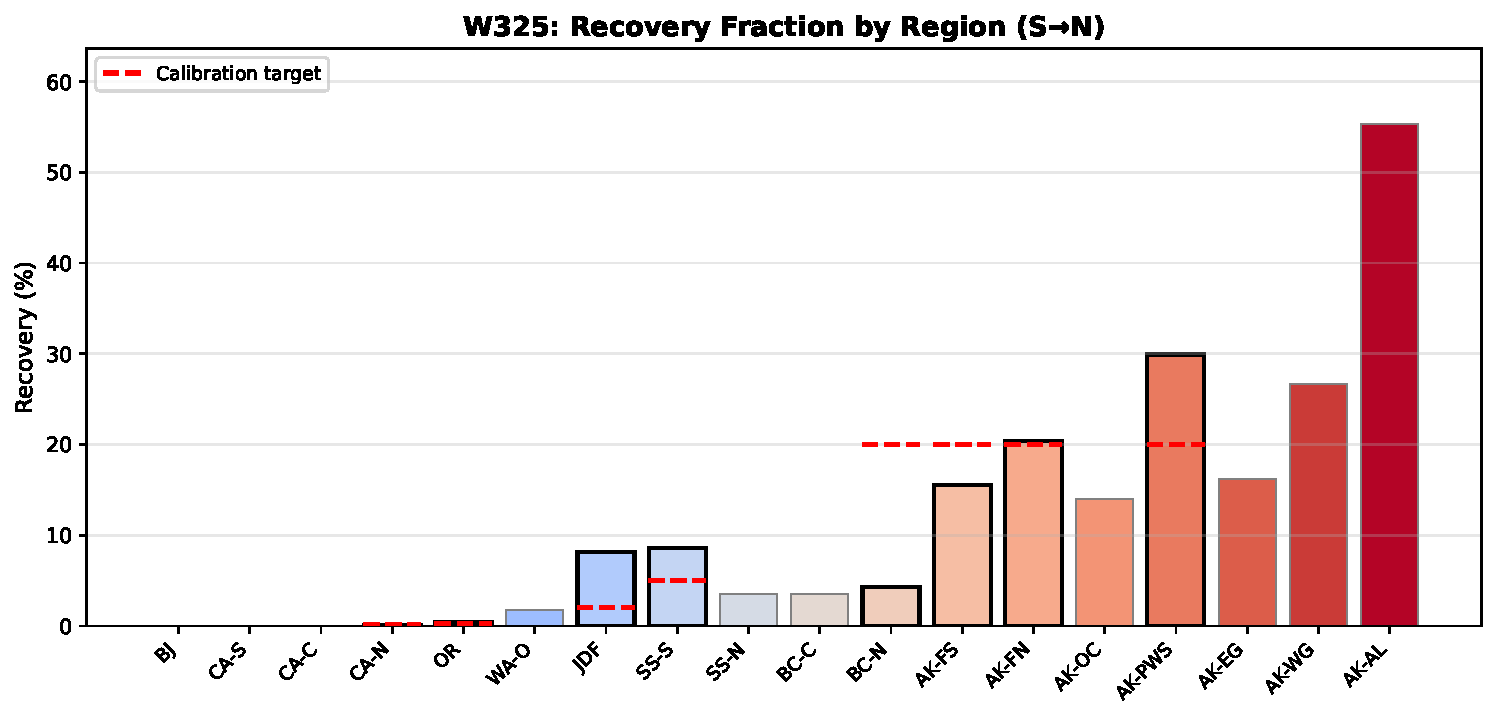
\includegraphics[width=0.85\textwidth]{figures/fig_3_5_recovery_map.pdf}
\caption{\textbf{Recovery fraction by region with calibration targets.}
Bars show simulated recovery; markers indicate targets.
AK-FN (20.4\% vs 20\%), OR (0.41\% vs 0.25\%), and CA-N (0.089\% vs 0.1\%) are on target.
BC-N is the worst miss: 4.3\% vs 20\% target ($4.7\times$ under).
JDF overshoots: 8.2\% vs 2\% target ($4.1\times$ over).
AK-PWS is moderately high at 29.9\% vs 20\%.}
\label{fig:recovery_map}
\end{figure}

%% ── Evolutionary Dynamics ───────────────────────────────────────────────
\section{Evolutionary Dynamics}

The spatial-temporal dynamics above raise a key question: how does the host population respond evolutionarily to sustained disease pressure?
W325 tracks three quantitative traits---resistance, tolerance, and recovery---plus pathogen cold-adaptation ($T_{\mathrm{vbnc}}$).

\begin{figure}[H]
\centering
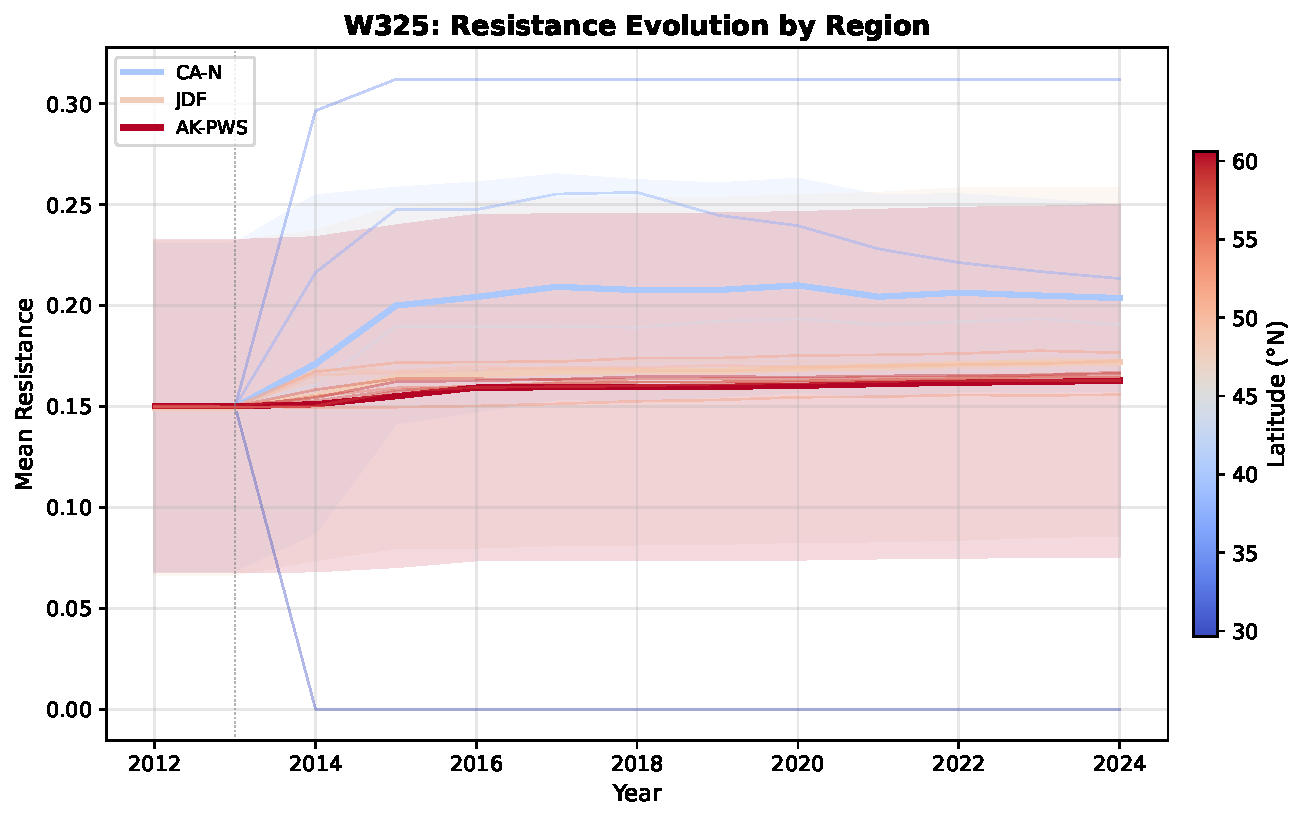
\includegraphics[width=0.85\textwidth]{figures/fig_4_1_resistance_evolution.pdf}
\caption{\textbf{Mean resistance trait by region over 13 years.}
All regions start at baseline $\sim$0.15.
CA-S undergoes a hard selective sweep, reaching 0.31 by year~3 (small surviving population, strong drift + selection).
Northern regions (AK) show gradual increase to 0.16--0.17 over the full simulation.
Mid-latitude regions (OR, WA-O, JDF, BC) show intermediate responses ($\sim$0.17--0.18).
The resistance response is strongest where disease mortality is most intense relative to population size.}
\label{fig:resistance}
\end{figure}

\begin{figure}[H]
\centering
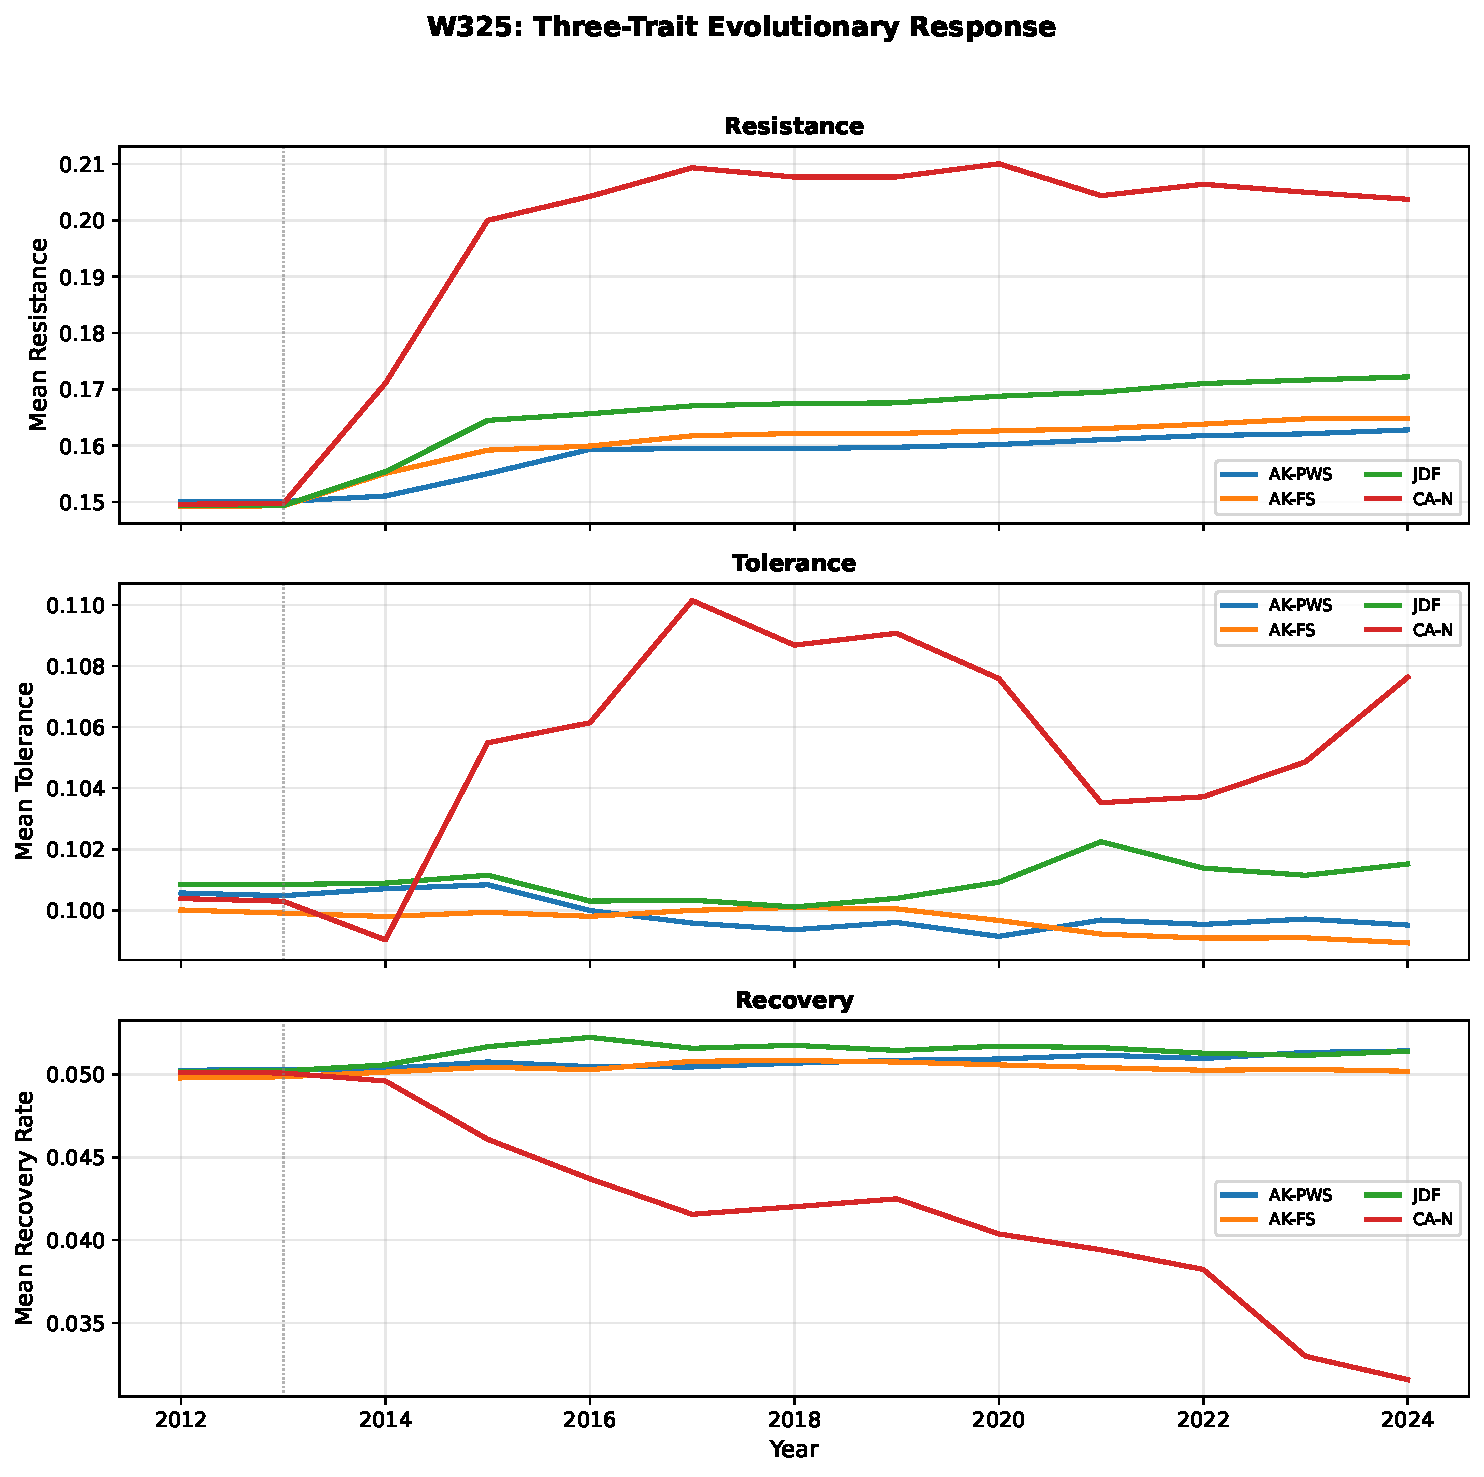
\includegraphics[width=\textwidth]{figures/fig_4_2_three_trait_panel.pdf}
\caption{\textbf{Three-trait evolutionary panel: resistance, tolerance, and recovery.}
Resistance (left) shows clear directional selection across all regions.
Tolerance (center) remains near baseline ($\sim$0.10) with no consistent directional change.
Recovery trait (right) is similarly static at $\sim$0.05.
This confirms resistance as the dominant adaptive axis: disease-induced mortality selects for resistance, not tolerance or faster recovery.
The lack of tolerance response may reflect weak selection gradients or genetic constraints on this trait.}
\label{fig:three_trait}
\end{figure}

\begin{figure}[H]
\centering
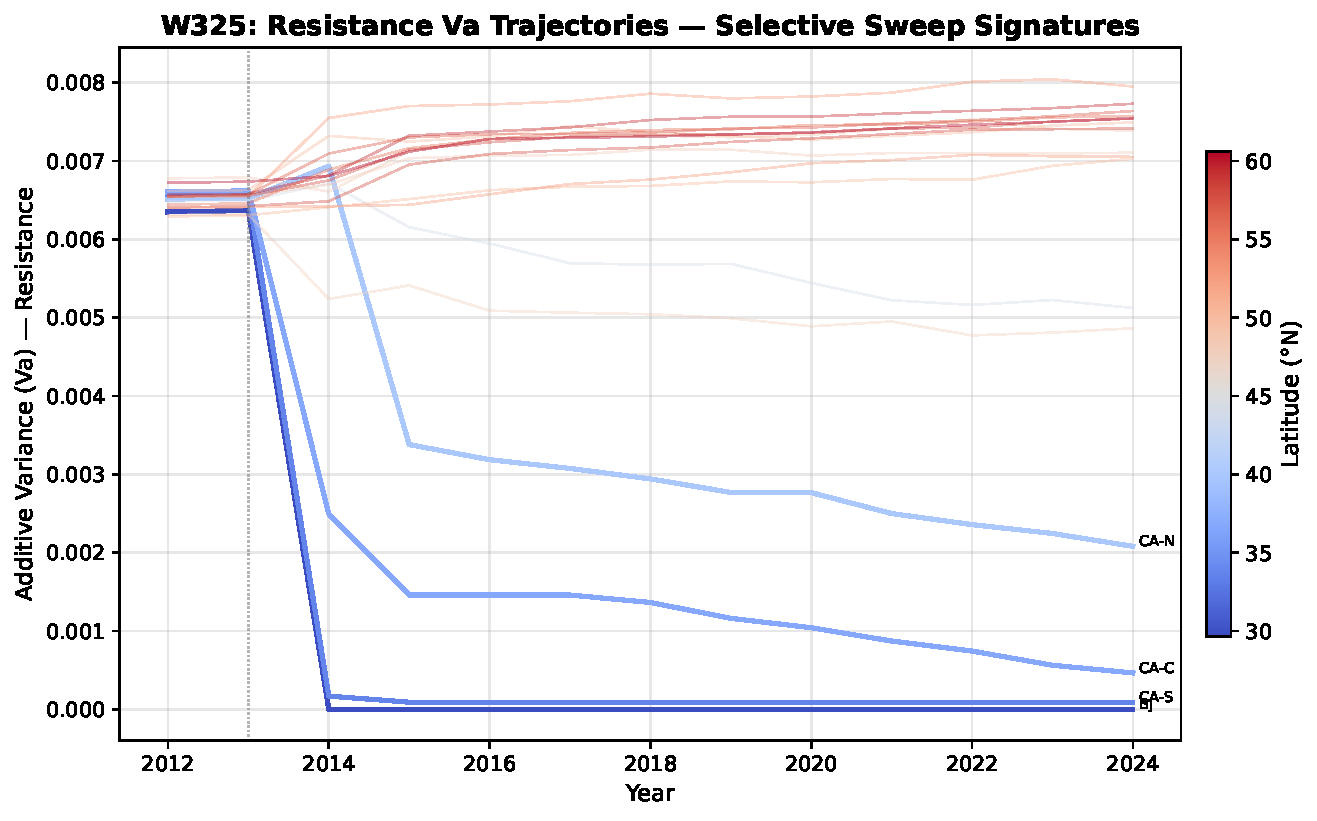
\includegraphics[width=0.85\textwidth]{figures/fig_4_3_va_trajectory.pdf}
\caption{\textbf{Additive genetic variance ($V_A$) trajectories for resistance.}
Southern regions (CA-S, CA-C) lose $V_A$ rapidly after year~2, consistent with selective sweeps or bottleneck-driven fixation.
Northern regions (AK) show slightly increasing $V_A$ ($\sim$0.0065 to 0.0075), indicating ongoing polygenic selection without fixation.
Mid-latitude regions are intermediate.
The $V_A$ pattern diagnoses the nature of selection: southern hard sweeps vs.\ northern sustained polygenic response.}
\label{fig:va}
\end{figure}

\begin{figure}[H]
\centering
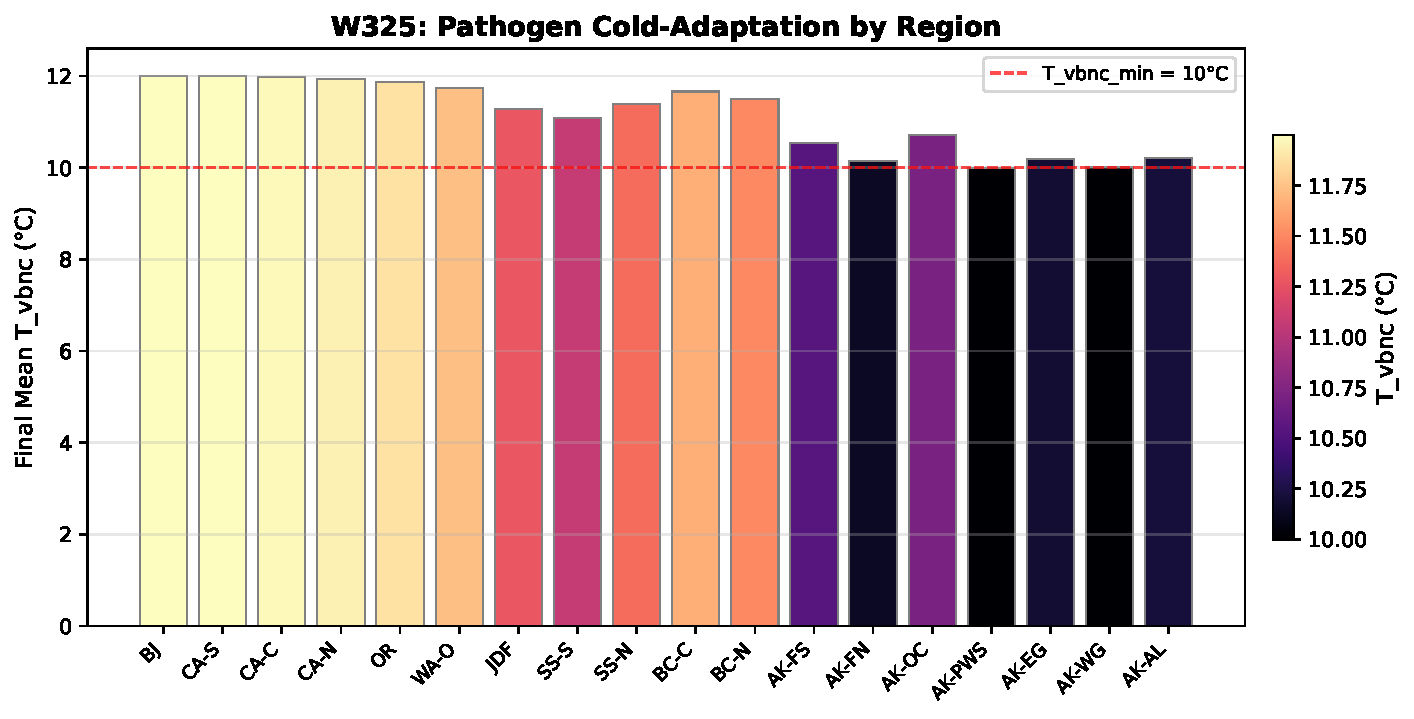
\includegraphics[width=0.85\textwidth]{figures/fig_4_4_pathogen_evolution.pdf}
\caption{\textbf{Pathogen cold-adaptation: final mean $T_{\mathrm{vbnc}}$ by region.}
$T_{\mathrm{vbnc}}$ decreases from $\sim$12$^\circ$C in southern regions to 10.0$^\circ$C in AK-PWS and AK-WG, hitting the $T_{\mathrm{vbnc,min}}=10^\circ$C floor.
This latitudinal gradient indicates pathogen adaptation to colder waters: strains that can remain active at lower temperatures are selected in northern environments.
The floor at 10$^\circ$C prevents further cold-adaptation, which may contribute to limiting disease severity in the coldest Alaska regions.}
\label{fig:pathogen}
\end{figure}

%% ── Calibration Performance ─────────────────────────────────────────────
\section{Calibration Performance}

With the dynamics and evolutionary context established, we turn to the core question: how well does W325 match empirical recovery targets?

\begin{figure}[H]
\centering
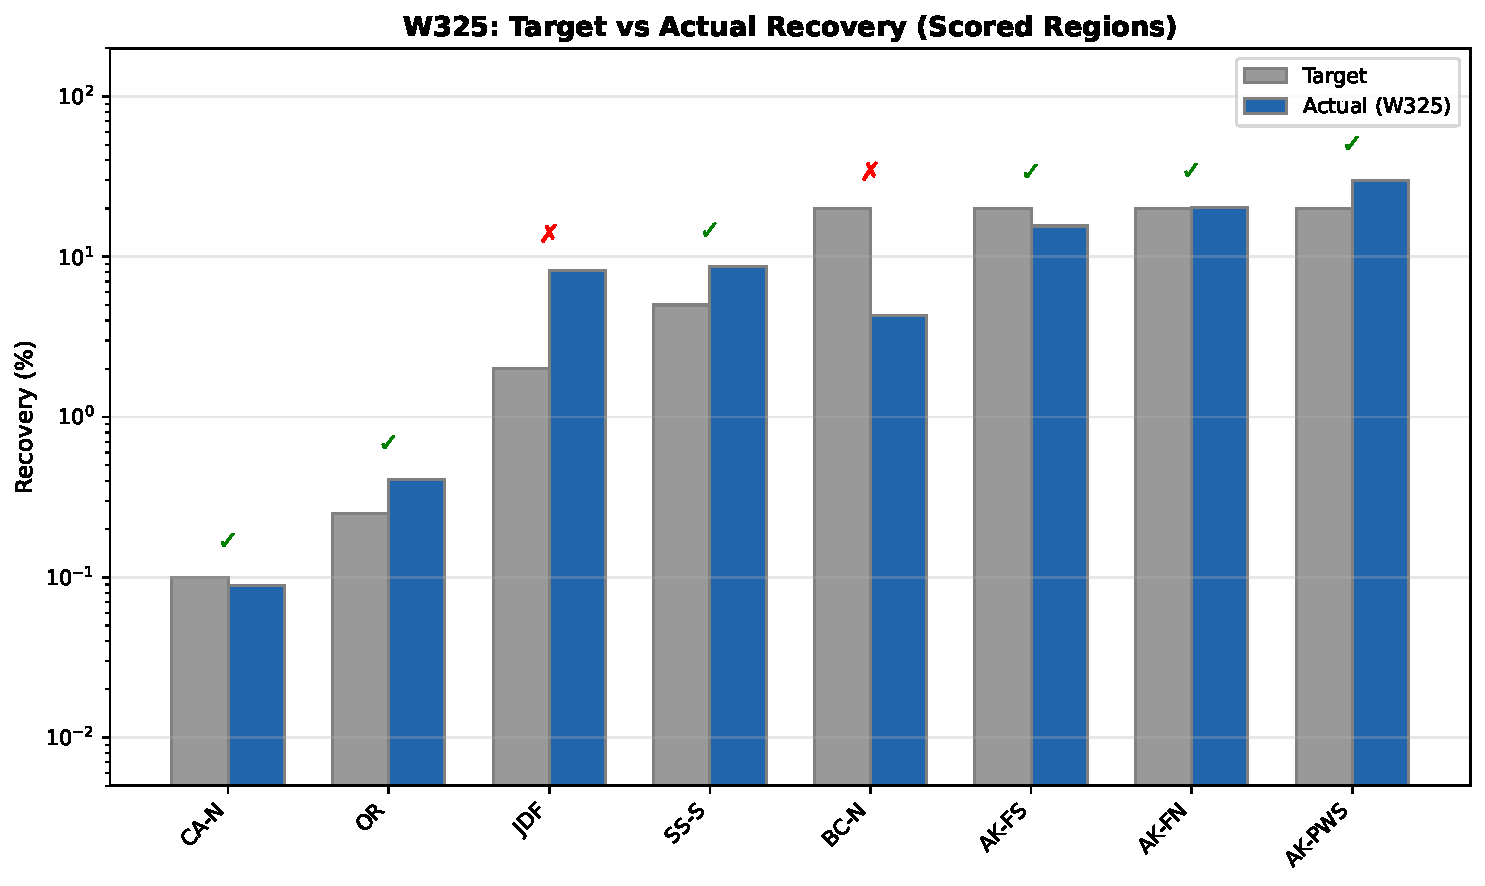
\includegraphics[width=0.85\textwidth]{figures/fig_5_1_recovery_vs_targets.pdf}
\caption{\textbf{Simulated vs.\ target recovery for all eight scored regions.}
Points near the 1:1 line indicate good calibration.
AK-FN, OR, and CA-N cluster tightly on the diagonal.
BC-N and JDF are the clear outliers: BC-N falls far below target (4.3\% vs 20\%), JDF far above (8.2\% vs 2\%).
AK-PWS and SS-S are moderately above their targets.
AK-FS is slightly under (15.5\% vs 20\%).}
\label{fig:recovery_targets}
\end{figure}

\begin{figure}[H]
\centering
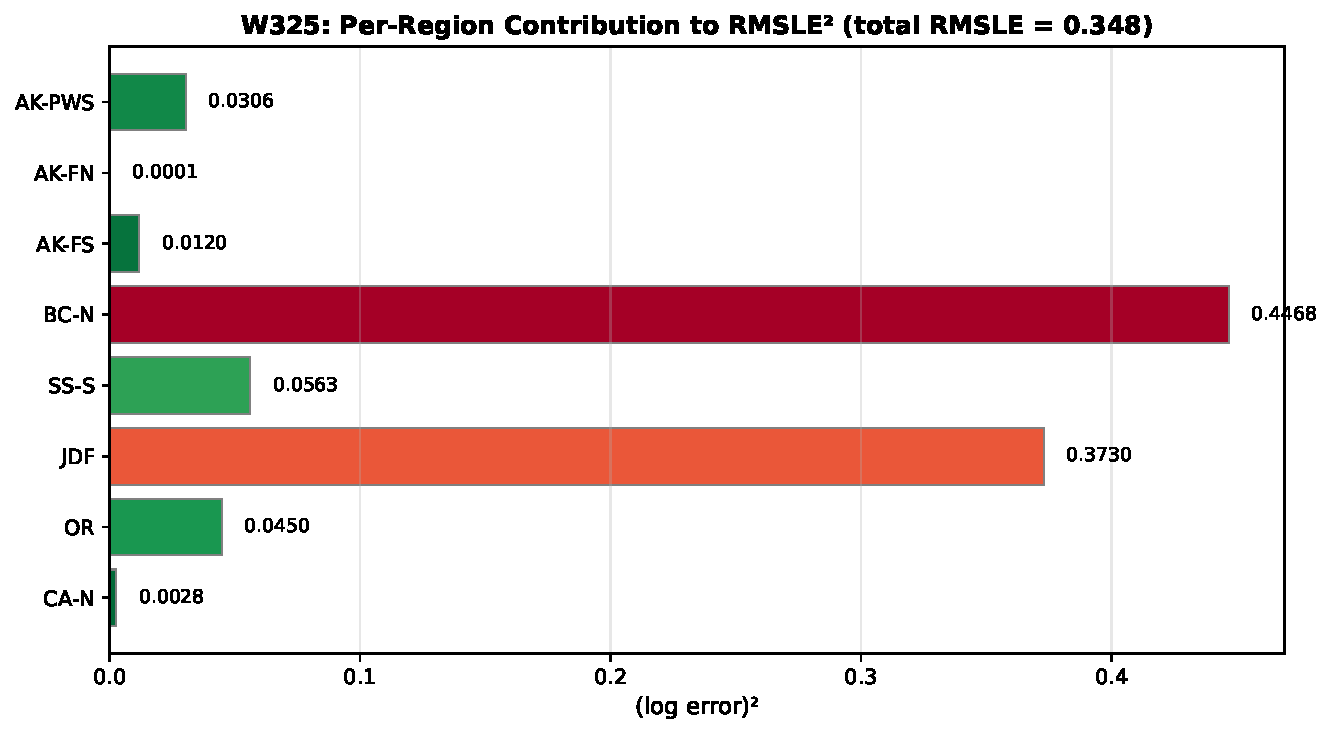
\includegraphics[width=0.85\textwidth]{figures/fig_5_2_scoring_breakdown.pdf}
\caption{\textbf{Per-region RMSLE$^2$ contribution to total error.}
BC-N contributes 0.447 (46\% of total) and JDF contributes 0.373 (39\%).
Together these two regions account for 85\% of the total squared log-error (0.820 of 0.967 total).
SS-S (0.056), OR (0.045), and AK-PWS (0.031) contribute modestly.
AK-FS (0.012), CA-N (0.003), and AK-FN ($<$0.001) are negligible.
\emph{Any parameter sweep targeting RMSLE reduction must primarily address BC-N and JDF.}}
\label{fig:scoring}
\end{figure}

\begin{table}[H]
\centering
\small
\caption{Calibration scorecard for W325. RMSLE\,=\,0.348.}
\label{tab:scorecard}
\begin{tabular}{lrrrccc}
\toprule
\textbf{Region} & \textbf{Target (\%)} & \textbf{Actual (\%)} & \textbf{Log$^2$ Error} & \textbf{$\leq$2$\times$} & \textbf{$\leq$5$\times$} & \textbf{Status} \\
\midrule
AK-PWS & 20.0 & 29.9 & 0.031 & \color{okgreen}\checkmark & \color{okgreen}\checkmark & $1.5\times$ over \\
AK-FN  & 20.0 & 20.4 & $<$0.001 & \color{okgreen}\checkmark & \color{okgreen}\checkmark & \color{okgreen}on target \\
AK-FS  & 20.0 & 15.5 & 0.012 & \color{okgreen}\checkmark & \color{okgreen}\checkmark & slightly under \\
BC-N   & 20.0 &  4.3 & 0.447 & \color{alertred}$\times$ & \color{okgreen}\checkmark & \color{alertred}$4.7\times$ under \\
SS-S   &  5.0 &  8.6 & 0.056 & \color{okgreen}\checkmark & \color{okgreen}\checkmark & $1.7\times$ over \\
JDF    &  2.0 &  8.2 & 0.373 & \color{alertred}$\times$ & \color{okgreen}\checkmark & \color{alertred}$4.1\times$ over \\
OR     &  0.25 &  0.41 & 0.045 & \color{okgreen}\checkmark & \color{okgreen}\checkmark & \color{okgreen}within $2\times$ \\
CA-N   &  0.1 & 0.089 & 0.003 & \color{okgreen}\checkmark & \color{okgreen}\checkmark & \color{okgreen}on target \\
\bottomrule
\end{tabular}
\end{table}

%% ── Conclusions & Next Steps ────────────────────────────────────────────
\section{Conclusions \& Next Steps}

W325 achieves RMSLE\,=\,0.348, a 47\% improvement over the previous best (W294, 0.655).
The two gradient-breaking mechanisms---$\delta_{\mathrm{env}}(T)$ and $P_{\mathrm{env}}$-gated recovery---are working:
southern regions that previously recovered too strongly (OR, CA-N) now match targets closely.

\textbf{What's working:}
\begin{itemize}[nosep,leftmargin=1.5em]
  \item Latitudinal gradient structure is correct: southern extirpation, mid-latitude intermediate, northern persistence.
  \item Three regions are on target: AK-FN (20.4\%), OR (0.41\%), CA-N (0.089\%).
  \item Southern suppression is effective: CA-S recovery $<$0.002\%, CA-C $\approx$ 0.01\%.
  \item Evolutionary dynamics are biologically plausible: resistance-dominated selection, pathogen cold-adaptation.
\end{itemize}

\textbf{What's not working:}
\begin{itemize}[nosep,leftmargin=1.5em]
  \item \textbf{BC-N} recovers to only 4.3\% vs.\ 20\% target. The $P_{\mathrm{env}}$-gated recovery or high $\alpha_{\mathrm{self,fjord}}=0.5$ may be over-suppressing BC fjord recruitment. BC-N has 75 nodes but only 3,144 final individuals (42 per node).
  \item \textbf{JDF} recovers to 8.2\% vs.\ 2\% target. As a semi-enclosed water body, JDF may need stronger self-retention ($\alpha_{\mathrm{self}}$) to maintain higher pathogen loads, or $\delta_{\mathrm{env,warm}}$ could be increased for temperate enclosed waters.
  \item \textbf{AK-PWS} is 1.5$\times$ over target (29.9\% vs 20\%). The $K_{\mathrm{half}}$ reduction to 800K may have been too aggressive---raising it back toward 1M could dampen Alaska recovery.
  \item \textbf{Arrival timing} is 10.4 months early on average for northern regions. The wavefront propagates too quickly.
\end{itemize}

\textbf{Recommended parameter adjustments for next sweep:}
\begin{enumerate}[nosep,leftmargin=1.5em]
  \item Reduce $\alpha_{\mathrm{self,fjord}}$ for BC regions (try 0.3) to increase larval import and boost BC-N recovery.
  \item Increase JDF-specific mortality or pathogen retention to suppress JDF recovery.
  \item Test $K_{\mathrm{half}} \in \{900\mathrm{K}, 1.0\mathrm{M}\}$ to moderate AK-PWS overshoot.
  \item Reduce $D_P$ from 300 to 200 to slow wavefront propagation and improve arrival timing.
  \item Consider region-specific $\delta_{\mathrm{env}}$ scaling for semi-enclosed vs.\ open coast.
\end{enumerate}

%% ── Appendix ────────────────────────────────────────────────────────────
\appendix
\section{Report Card}

\begin{figure}[H]
\centering
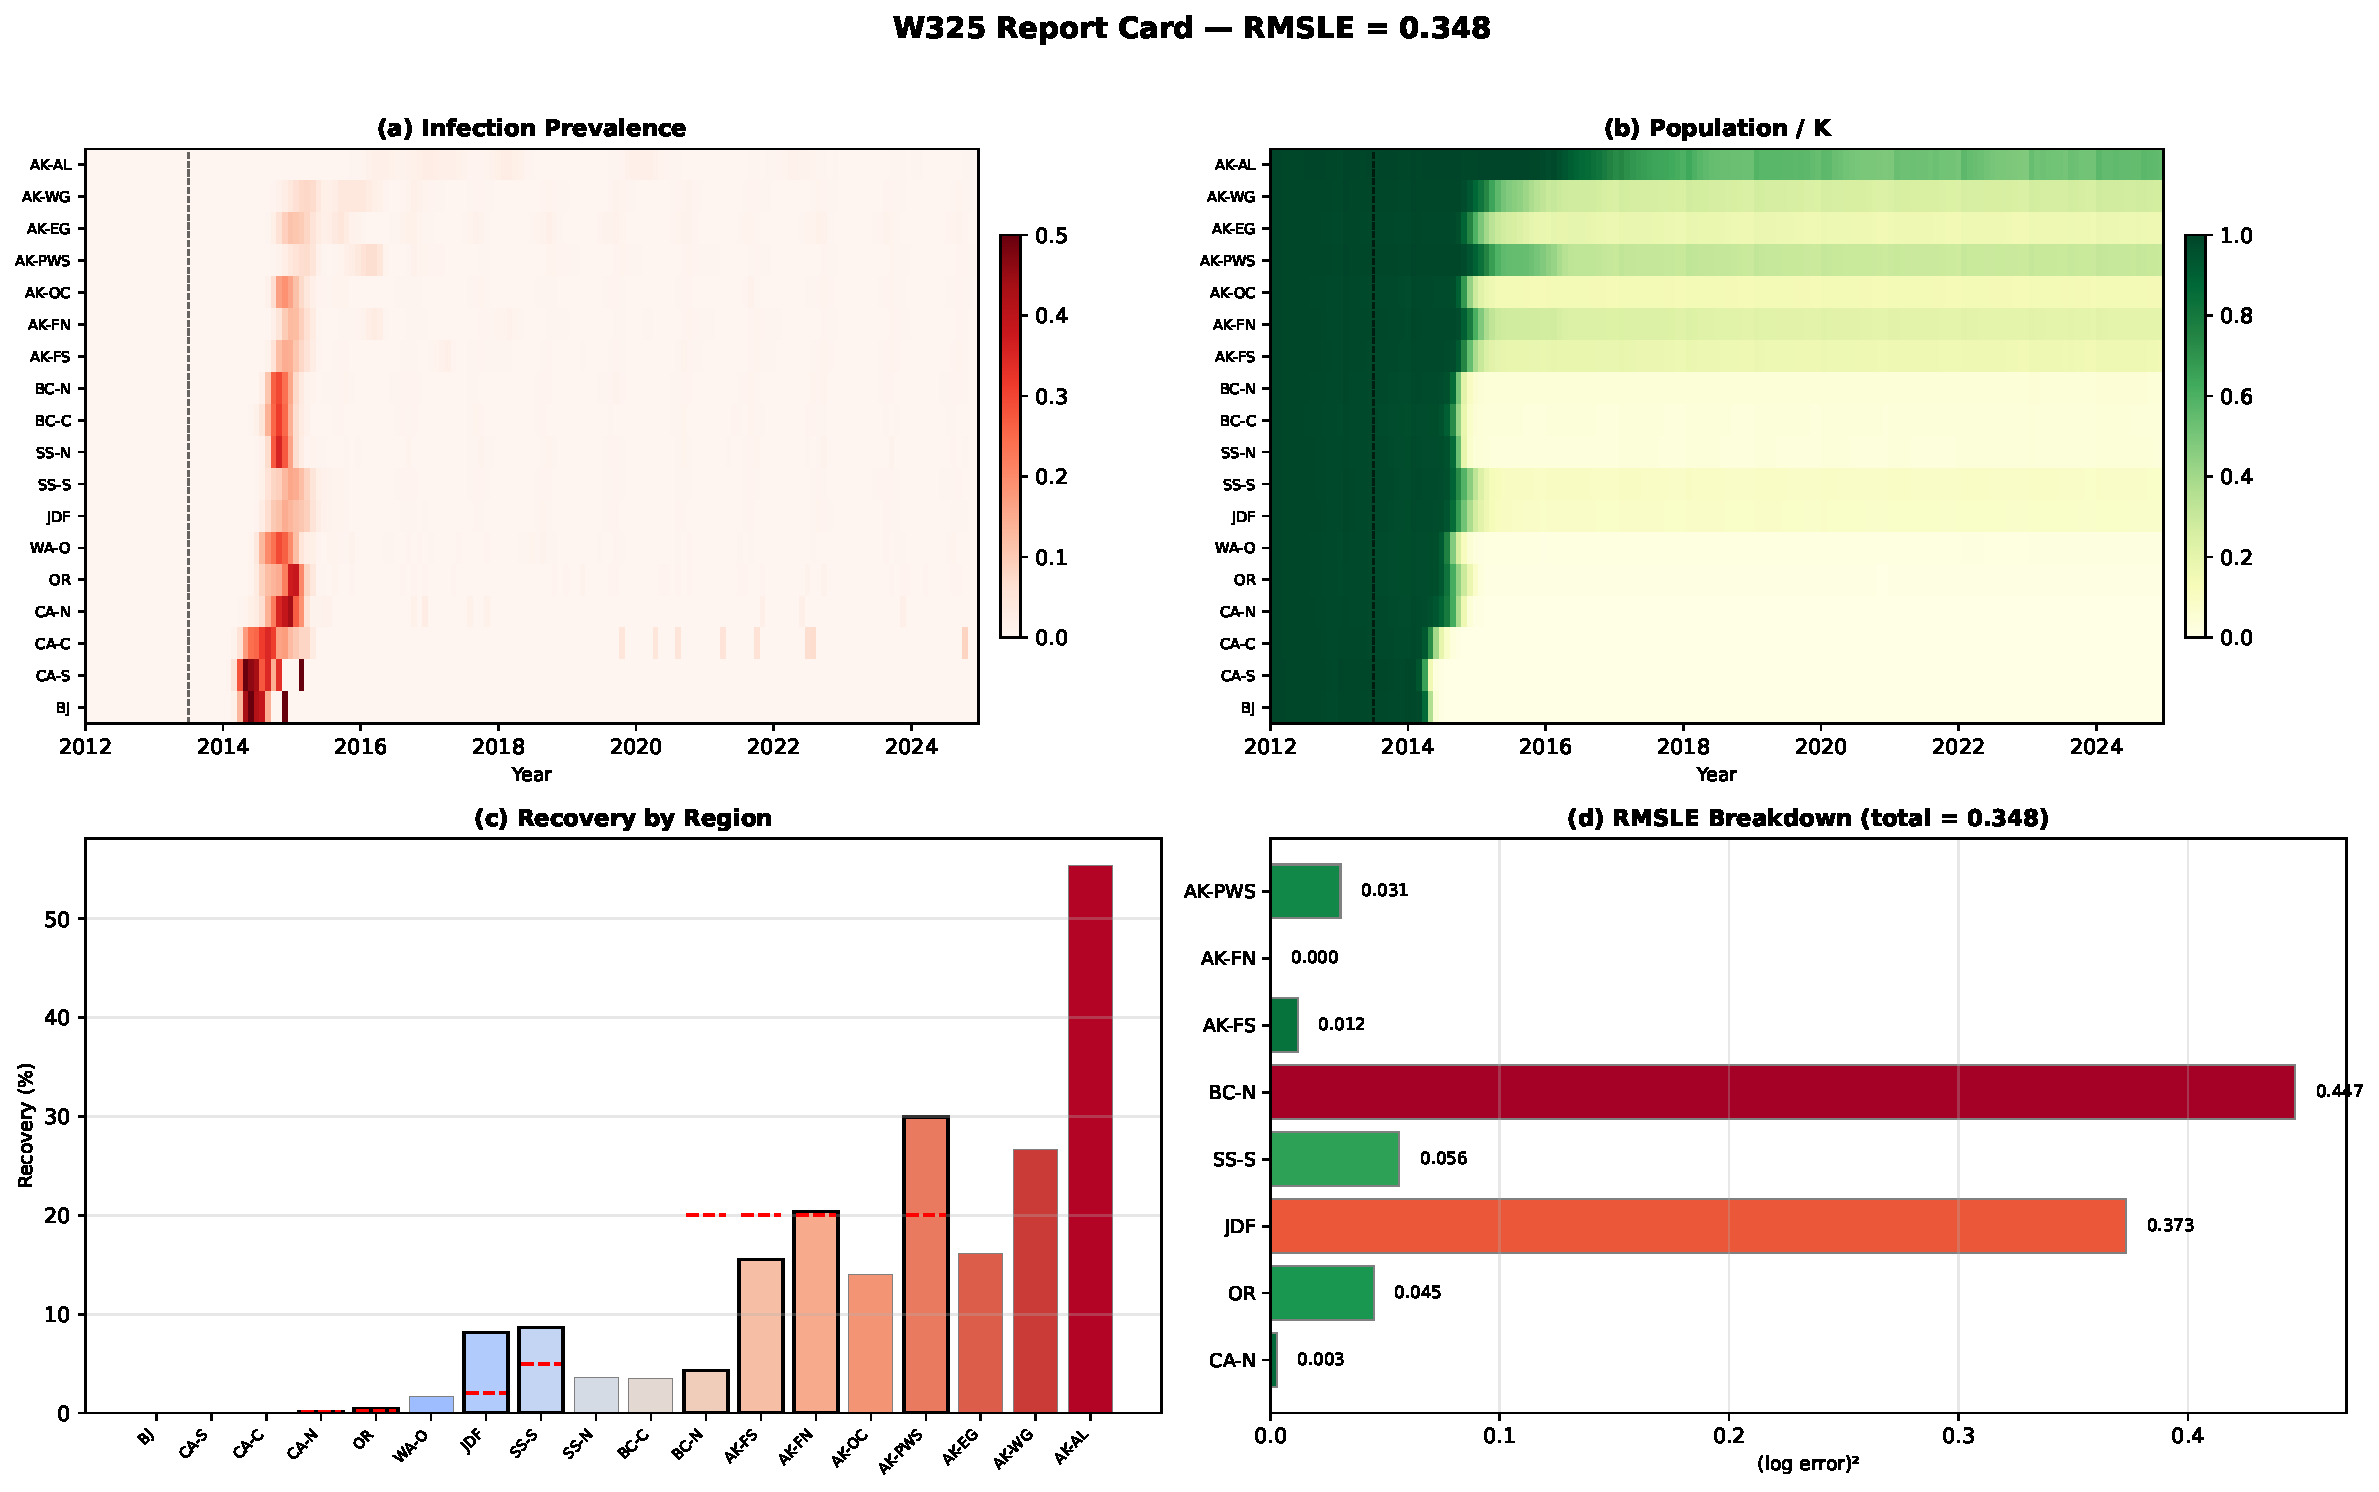
\includegraphics[width=\textwidth]{figures/fig_A_1_report_card.pdf}
\caption{\textbf{W325 report card: 2$\times$2 composite summary.}
Top-left: infection heatmap showing wavefront progression.
Top-right: population heatmap showing crash-recovery pattern.
Bottom-left: recovery vs.\ targets for scored regions.
Bottom-right: per-region scoring breakdown.
W325 achieves RMSLE\,=\,0.348 with 6/8 regions within 2$\times$ and 8/8 within 5$\times$ of targets.}
\label{fig:report_card}
\end{figure}

\end{document}
